\section{Worker loading}
To run the workload files we loaded sections of 3300 transactions into workers in a round-robin manner.
By measuring the total number of transaction in a worker's backlog at each loading cycle we could determine the limits of our round-robin loading method.

\subsection{Worker backlog analysis}

\begin{figure}[tbph]
  \centering
  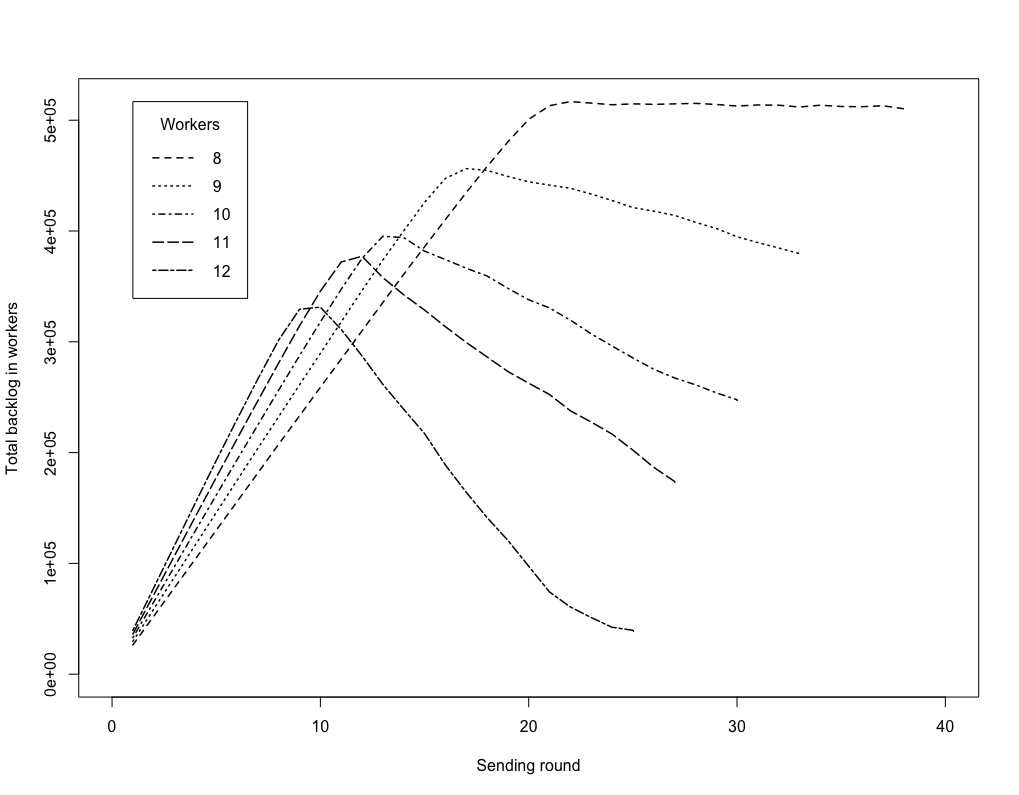
\includegraphics[width=0.9\linewidth]{graphics/backlog_by_workers}
  \caption{Total worker backlog for 1000 user workload}
  \label{fig:backlog-total}
\end{figure}

The curves in Figure~\ref{fig:backlog-total} have two distinct parts: an upward slope that becomes steeper as the number of workers before coming to a maximum and either plateauing, as with eight workers; decreasing at a fixed rate, as with nine to eleven workers, or; decreasing and leveling out, as with twelve workers.
It's important to note that the x-axis represents loading cycles and not a uniform time scale.
Round robin loading cycle times increase as the number of workers increases.

The slope of the curve represents the ratio of transactions coming in to a worker over transactions completed between successive cycles.
Essentially, this is
\begin{equation*}
  {\SI{3300}{transactions per cycle} \times \si{cycles per second} \over \si{transactions per second}}
\end{equation*}
The peak in the curves occurs when the system has retrieved a full load of quotes the transactions per second increases drastically.
For eight workers, the slope is approximately 1, indicating that the input and output rates are equal.
The work in~\ref{sec:worker-scaling-results} indicates that the transaction input rate must be approximately \SI{3600}{transactions per second} for each worker.
As the number of workers increases, the number of transactions per second for a worker stays (mostly) constant but the cycles per second decreases.
The leveling off with twelve workers indicates that the workers are starved for transactions near the end of the run.

The change in the rising slopes is also affected by the increased cycle time but the correlation is less direct.
During loading, the transactions per second is significantly lower than 3300 and constant regardless of the number of workers.
The slope increases with the number of workers because the capacity for transactions in the system increases (i.e. each worker has its own cache).
As the cycle times become longer this decreases the slope.

\subsection{Worker starvation analysis}

\begin{figure}[tbph]
  \centering
  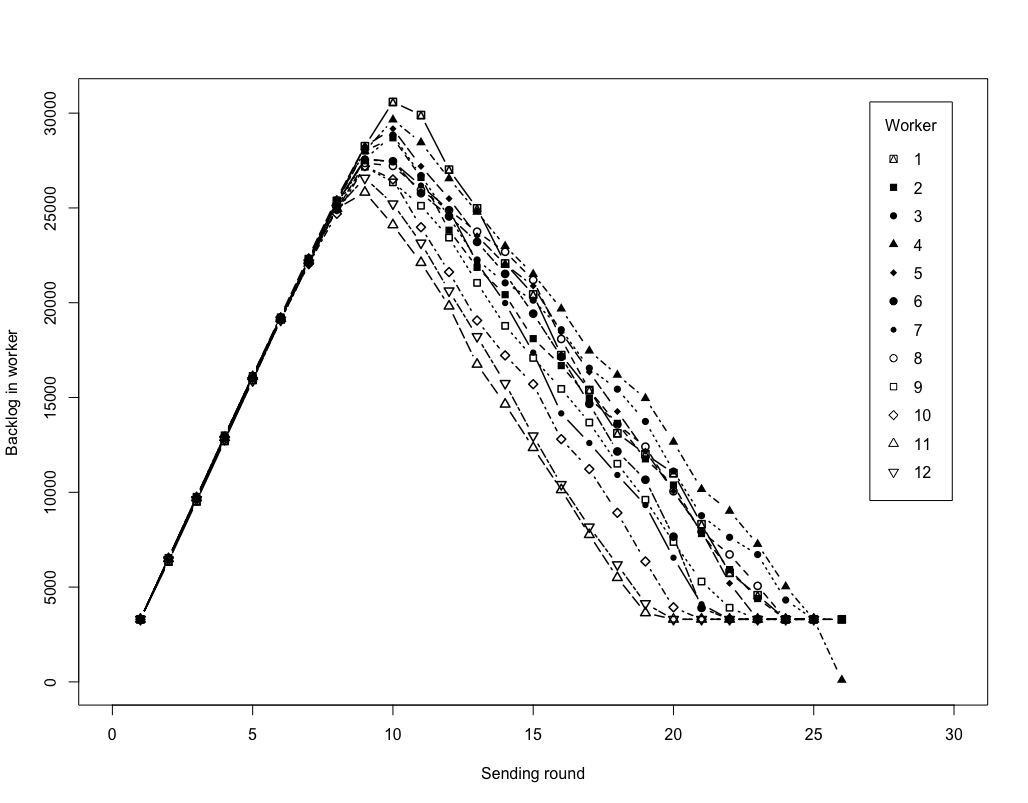
\includegraphics[width=0.85\linewidth]{../../data/worker-load/backlog_12w}
  \caption{Workers entering starvation during a 1000 user workload}
  \label{fig:backlog12w}
\end{figure}

Figure~\ref{fig:backlog12w} shows how workers entering starvation at different times.
All workers have identical backlogs up until the peak where higher-numbered workers operate at nominal TPS earlier.
This is because the low-numbered workers early in the round-robin cycle are ``alone'' for longer with the transaction list and are more likely to encounter uncached quotes.
High-numbered workers benefit from the pre-caching.
Unfortunately, they enter starvation approximately ten cycles before loading finishes and represent an inefficient use of resources.

The rates of descent are mostly uniform, with the exception of worker 4 (machine B133).
Consistently, this machine performed worse than its peers.
This could be the result of hardware aging and general, spooky ``cruft'' on the machine or a non-uniformity in the workload distribution.
The latter is unlikely since worker 4 was slow regardless of the total number of workers.

We did not undertake any tests with thirteen workers because of these results with twelve \textemdash{} adding more workers would cause the system to enter starvation earlier and would be a poor use of resources.

\subsection{Alternate solutions}
The ideal operating state is when the incoming and outgoing transaction rates are equal.
In order to achieve this state we would have to implement a feedback system with the transaction loader.
The number of backlogged transactions in a worker could change the number of transactions sent in a loading cycle.

Though not trivial, this is a very tractable solution.
However, we feel it would be overly specific to the testing environment.
Could an actually existing trading system exert backpressure on user loads to throttle demand? This seems unlikely, or at least one that would lead to frustrated users.
Further testing should involve a dynamic \textit{stream} of transactions that could exhibit richer behavior like cyclic demand cycles and surges.
Though the same risk of overfitting the prototype software to the test environment is present, the fidelity has increased and the solutions should be more generally applicable.
